%\subsection{Context and motivation of PhD}


\begin{frame}{Introduction}{Context and motivation of PhD}

\begin{block}{\textbf{Context and motivation}}
	\begin{minipage}[t]{0.48\linewidth}
		%\begin{itemize}
		%	\item \ac{DC} supply system architecture	
		%\end{itemize}
	%	\vspace{-1em}
		\begin{figure}[ht!]
			\centering
			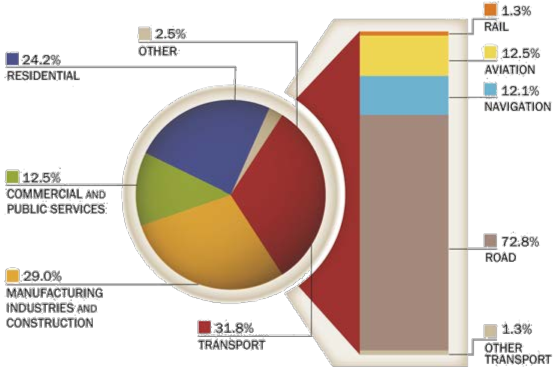
\includegraphics[width=0.93\textwidth,keepaspectratio]{figures/1.Intro/iea-uic-energy}
			\caption{Global Energy Consumption. \cite{iea-uic2016}.}
		\end{figure}
	\end{minipage}\hfill
	\begin{minipage}[t]{0.48\linewidth}
		%\begin{itemize}
		%	\item  50 Hz 25 kV supply system.
		
		%\end{itemize}
		\vspace{4.45em}
		\begin{figure}[ht!]
			\centering
			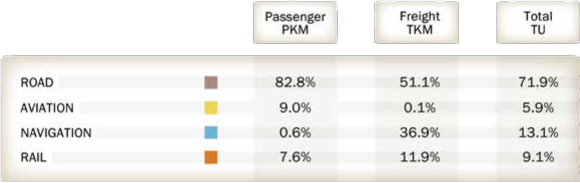
\includegraphics[width=\textwidth,keepaspectratio]{figures/1.Intro/iea-uic-share}
			\caption{Global Transportation Share. \cite{iea-uic2016}.}
		\end{figure}
		
	\end{minipage}
\end{block}
\end{frame}

%%%%%%%%%%%%%%%%%%%%%%%%%%%%%%%%%%%%%%%%%%%%%%%%%%%%%%%%%%%%%%%%%%%%%%%%%%%%%%%%%%%%%

\begin{frame}{Introduction}{Context and motivation of PhD}
\begin{block}{\textbf{Shift2Rail Framework - Main Goal}}
	\begin{itemize}
		%	\setlength\itemsep{-0.5em}
		\item 1. Cutting the life-cycle cost of railway transport by, at least, 50\%;
		\item 2. Doubling the railway capacity;
		\item 3. Increasing the reliability and punctuality by 50\%, at least.
	\end{itemize}
	
\end{block}
\end{frame}
%%%%%%%%%%%%%%%%%%%%%%%%%%%%%%%%%%%%%%%%%%%%%%%%%%%%%%%%%%%%%%%%%%%%%%%%%%%%%%%%%%%%%

\begin{frame}{Introduction}{Context and motivation of PhD}
%\begin{block}{\textbf{Shift2Rail Framework - Time Targets}}
%Complementary, the time target goals are the establishment of a framework, by 2020, for a European multimodal transport system for the passenger rail, freight and for the urban mobility. By 2030 is expected to triple the length of the existing high-speed passenger rail network, 30\% of the road freight over 300 km should shift to rail or waterborne transport and achieve a CO2-free city logistics in major urban centers. By 2050, the medium-distance passenger transport should go by rail and high-speed rail, with the connection of all core network airports to the high-speed railway network. On the freight is expected to have all seaports connected to the rail freight transport system and on the urban mobility, the "conventionally-fueled" cars will not have place in cities by 2050, \cite{shift2rail2015}.
\begin{figure}[ht!]
	\centering
	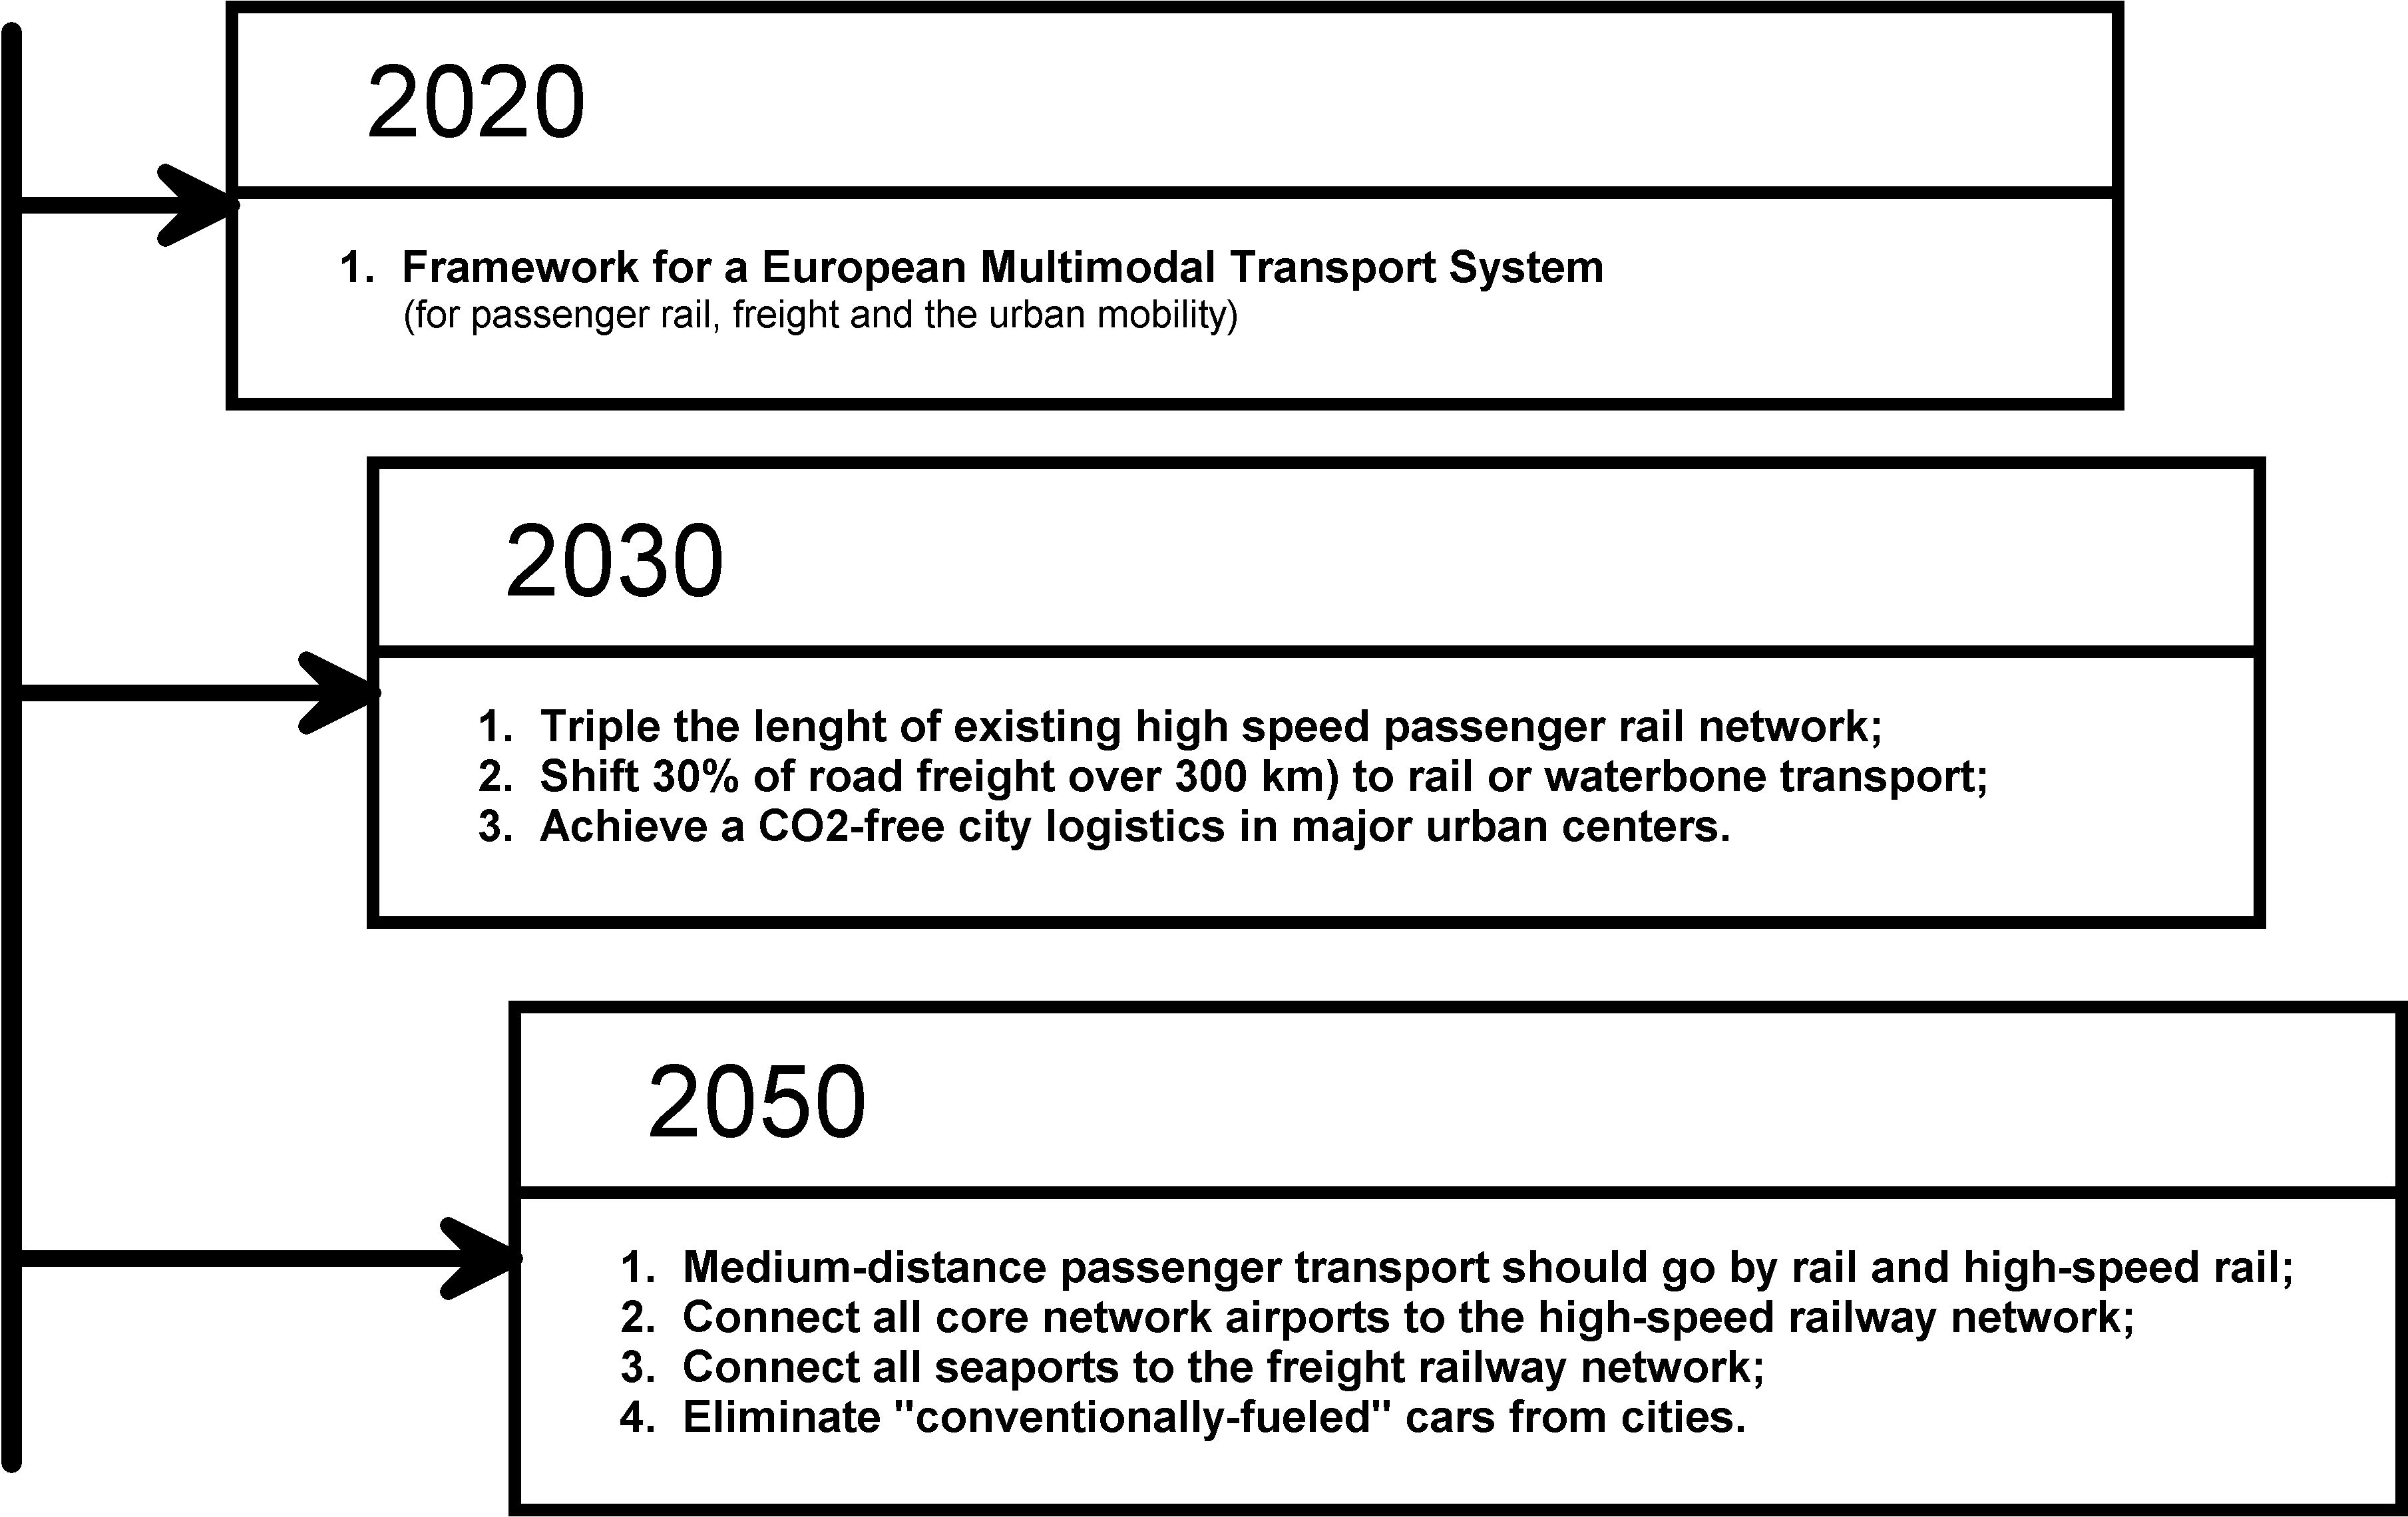
\includegraphics[width=0.7\textwidth,keepaspectratio]{figures/1.Intro/time_targets}
	\caption{Shift2Rail Framework - Time Targets. \cite{shift2rail2015}}
\end{figure}

%\end{block}
\end{frame}
%%%%%%%%%%%%%%%%%%%%%%%%%%%%%%%%%%%%%%%%%%%%%%%%%%%%%%%%%%%%%%%%%%%%%%%%%%%%%%%%%%%%%





\begin{frame}{Introduction}{Context and motivation of PhD}
%\begin{minipage}[t]{0.5\linewidth}
	\begin{figure}[ht!]
	\centering
	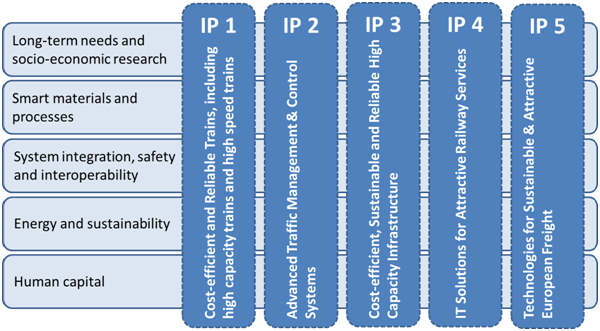
\includegraphics[width=0.6\textwidth,keepaspectratio]{figures/1.Intro/IPs}
	\caption{Shift2Rail Framework - Innovation Programmes. \cite{shift2rail2015}}
	\end{figure}
%\end{minipage}\hfill
%\begin{minipage}[t]{0.48\linewidth}
\pause
\vspace{-1em}
	\begin{block}{\textbf{Smart Meter Demonstrator}}
	\begin{itemize}
		\setlength\itemsep{0em}
		\item Towards detailed monitoring and supervision of energy flows;
	\end{itemize}
	\end{block}
	%
		%	The \ac{S2R} carries five innovation programmes, as presented in figure \ref{fig:ips}. Framed on the S2R \ac{IP3} with the focus on the ”Cost efficient and reliable infrastructure”, it is proposed the development of a \ac{SMD} that achieves a detailed monitoring and supervision of various energy flows on the premises of embracing the entire \ac{RTS}.
	%
%\end{minipage}



%\begin{figure}[h!]
%	\centering
%	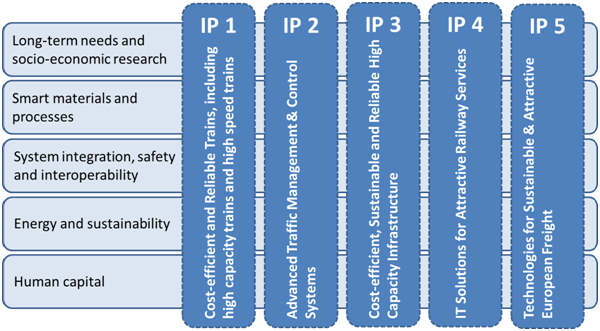
\includegraphics[width=0.60\textwidth,keepaspectratio]{figures/1.Intro/IPs}
%	\caption{Shif2Rail Innovation Programs. }
%\end{figure}
\end{frame}
%%%%%%%%%%%%%%%%%%%%%%%%%%%%%%%%%%%%%%%%%%%%%%%%%%%%%%%%%%%%%%%%%%%%%%%%%%%%%%%%%%%%%



%\begin{frame}{Introduction}{Context and motivation of PhD}
 %\begin{block}{\textbf{Context and motivation}}
	
	
%	\begin{minipage}[t]{0.48\linewidth}
		%\begin{itemize}
		%	\item \ac{DC} supply system architecture	
		%\end{itemize}

%		\begin{figure}[ht!]
%			\centering
%			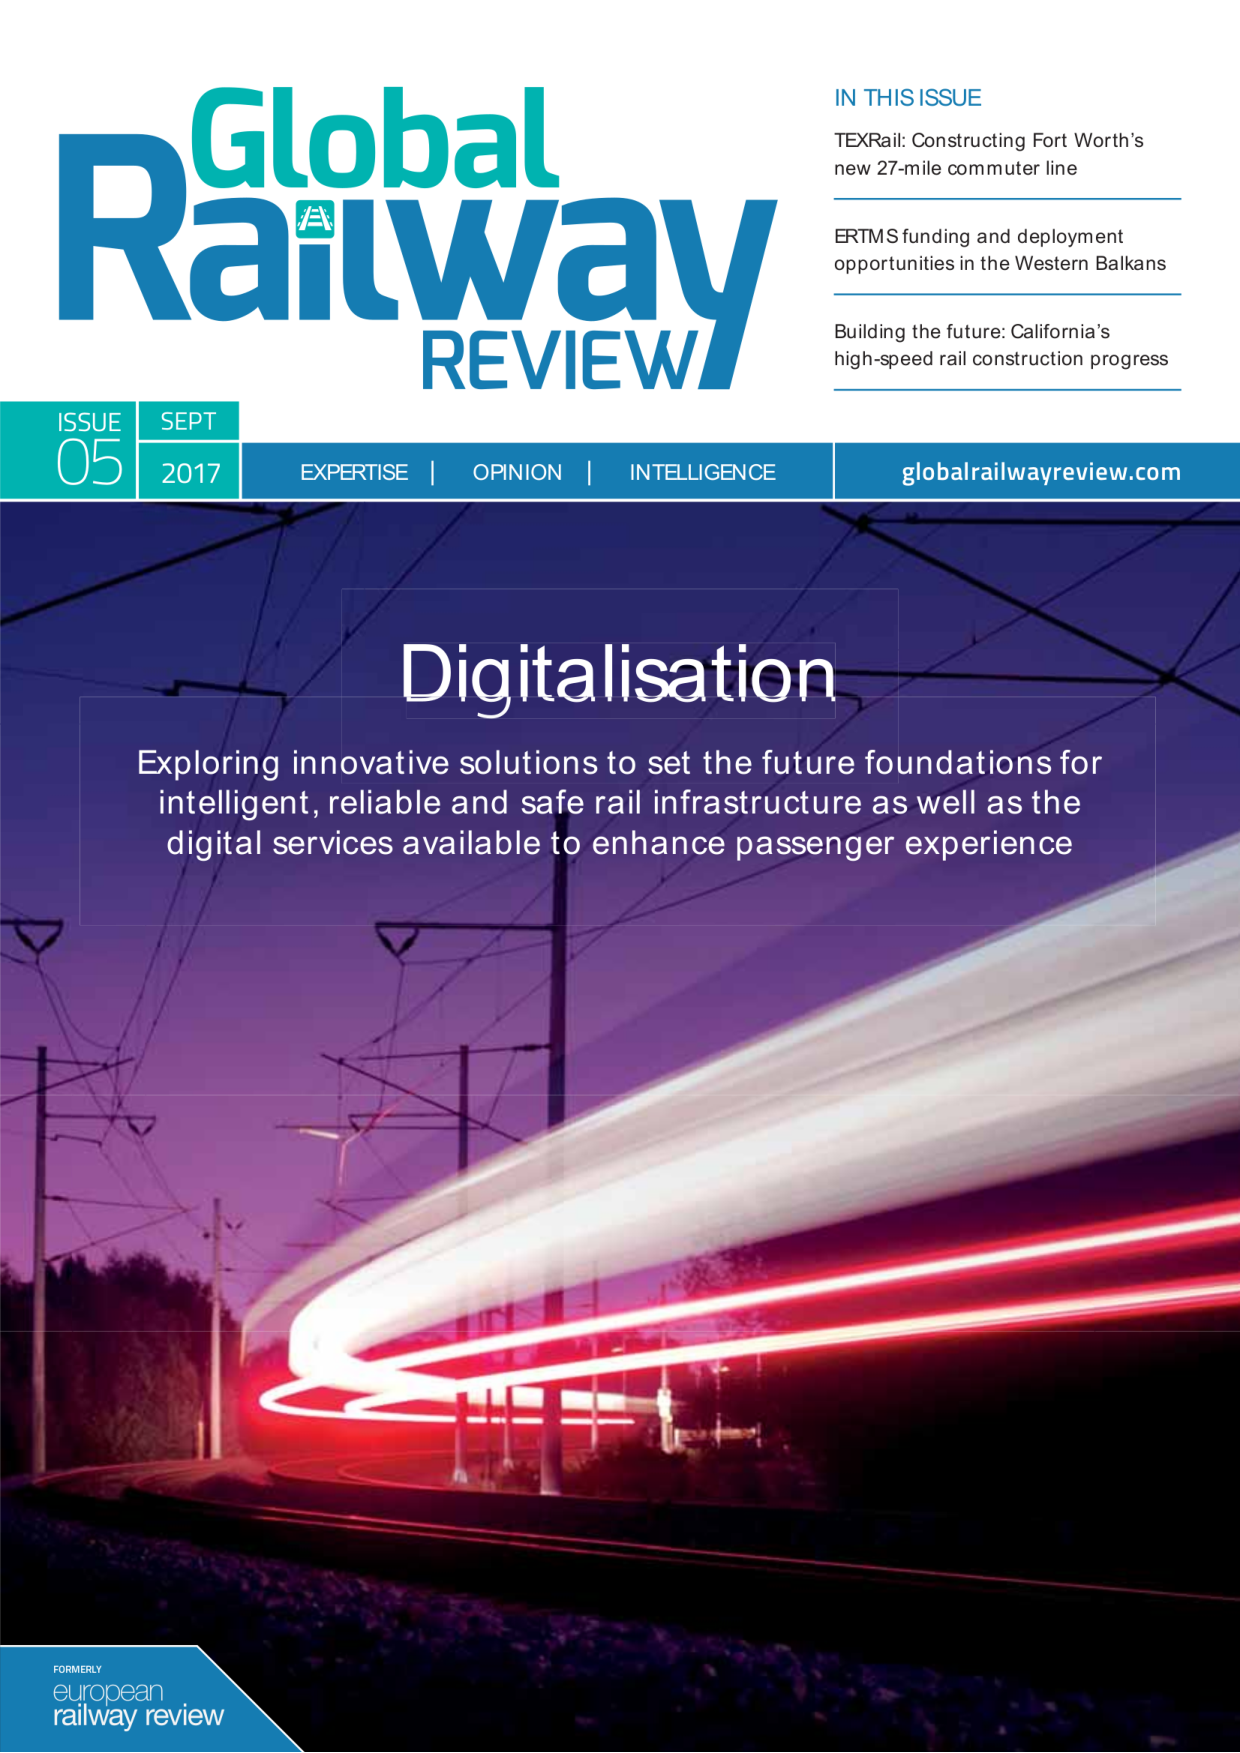
\includegraphics[width=0.5\textwidth,keepaspectratio]{figures/1.Intro/grr_magazine_10}
%			\caption{Front Page of Global Railway Review magazine.}
%		\end{figure}
%	\end{minipage}\hfill
%	\begin{minipage}[t]{0.48\linewidth}
		%\begin{itemize}
		%	\item  50 Hz 25 kV supply system.
		
		%\end{itemize}
%\vspace{2em}
%		\begin{figure}[ht!]
%			\centering
%			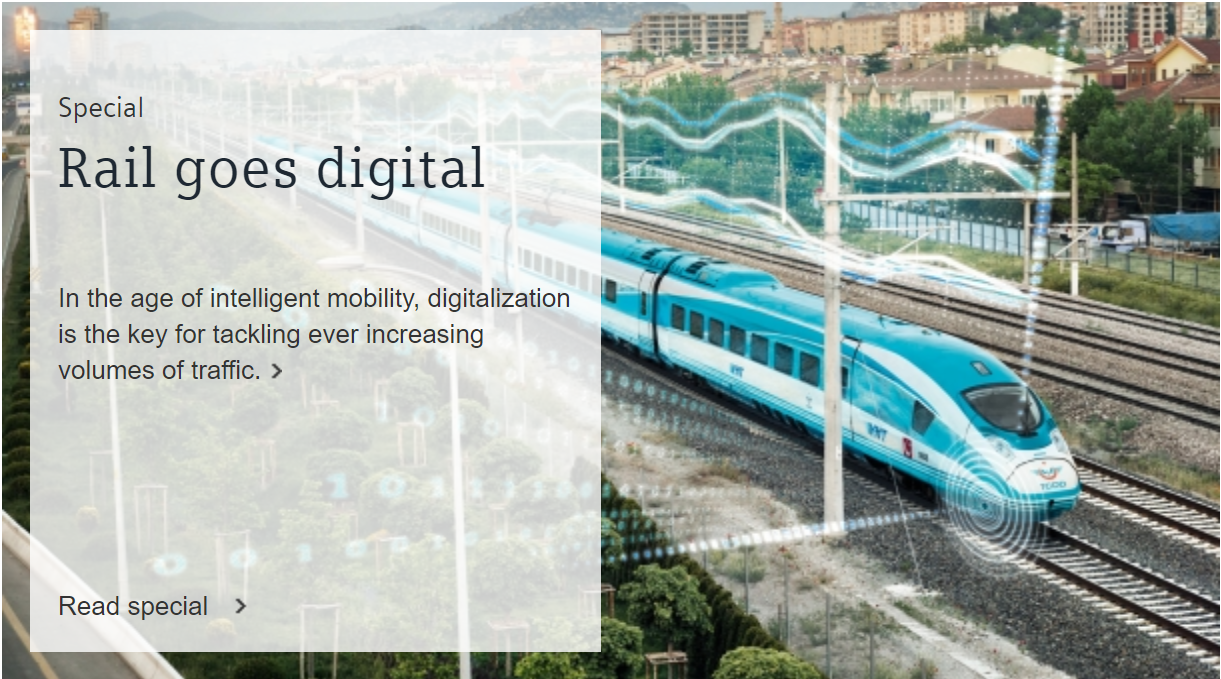
\includegraphics[width=1\textwidth,keepaspectratio]{figures/1.Intro/siemens}
%			\caption{Siemens Special Issue in InnoTrans Fair.}
%		\end{figure}
		
		
		
%	\end{minipage}
	
%\end{block}
%\end{frame}
%%%%%%%%%%%%%%%%%%%%%%%%%%%%%%%%%%%%%%%%%%%%%%%%%%%%%%%%%%%%%%%%%%%%%%%%%%%%%%%%%%%%%




%\subsection{Objectives}

\begin{frame}{Introduction}{Objectives}
\begin{block}{\textbf{Objectives}}
\begin{itemize}
	\setlength\itemsep{0em}
	
	\item	Research on \textbf{railway energy models}, and \textbf{development/implementation of a metering system} for railway power flow monitoring.
	This is expected to be based on a non-intrusive self-powered sensor node inserted into train power system.
	
	\item Research on \textbf{communication network models} for a \ac{RTS} wireless network with \textbf{validation through simulation frameworks}.
	\textbf{Development and implementation} of \ac{RTS} wireless network to store the energy information data of railway into central database.
	
	
\end{itemize}
\end{block}
\end{frame}
%%%%%%%%%%%%%%%%%%%%%%%%%%%%%%%%%%%%%%%%%%%%%%%%%%%%%%%%%%%%%%%%%%%%%%%%%%%%%%%%%%%%%